% Options for packages loaded elsewhere
\PassOptionsToPackage{unicode}{hyperref}
\PassOptionsToPackage{hyphens}{url}
%
\documentclass[
]{article}
\usepackage{lmodern}
\usepackage{amsmath}
\usepackage{ifxetex,ifluatex}
\ifnum 0\ifxetex 1\fi\ifluatex 1\fi=0 % if pdftex
  \usepackage[T1]{fontenc}
  \usepackage[utf8]{inputenc}
  \usepackage{textcomp} % provide euro and other symbols
  \usepackage{amssymb}
\else % if luatex or xetex
  \usepackage{unicode-math}
  \defaultfontfeatures{Scale=MatchLowercase}
  \defaultfontfeatures[\rmfamily]{Ligatures=TeX,Scale=1}
\fi
% Use upquote if available, for straight quotes in verbatim environments
\IfFileExists{upquote.sty}{\usepackage{upquote}}{}
\IfFileExists{microtype.sty}{% use microtype if available
  \usepackage[]{microtype}
  \UseMicrotypeSet[protrusion]{basicmath} % disable protrusion for tt fonts
}{}
\makeatletter
\@ifundefined{KOMAClassName}{% if non-KOMA class
  \IfFileExists{parskip.sty}{%
    \usepackage{parskip}
  }{% else
    \setlength{\parindent}{0pt}
    \setlength{\parskip}{6pt plus 2pt minus 1pt}}
}{% if KOMA class
  \KOMAoptions{parskip=half}}
\makeatother
\usepackage{xcolor}
\IfFileExists{xurl.sty}{\usepackage{xurl}}{} % add URL line breaks if available
\IfFileExists{bookmark.sty}{\usepackage{bookmark}}{\usepackage{hyperref}}
\hypersetup{
  pdftitle={Penalized Regression},
  hidelinks,
  pdfcreator={LaTeX via pandoc}}
\urlstyle{same} % disable monospaced font for URLs
\usepackage[margin=1in]{geometry}
\usepackage{color}
\usepackage{fancyvrb}
\newcommand{\VerbBar}{|}
\newcommand{\VERB}{\Verb[commandchars=\\\{\}]}
\DefineVerbatimEnvironment{Highlighting}{Verbatim}{commandchars=\\\{\}}
% Add ',fontsize=\small' for more characters per line
\usepackage{framed}
\definecolor{shadecolor}{RGB}{248,248,248}
\newenvironment{Shaded}{\begin{snugshade}}{\end{snugshade}}
\newcommand{\AlertTok}[1]{\textcolor[rgb]{0.94,0.16,0.16}{#1}}
\newcommand{\AnnotationTok}[1]{\textcolor[rgb]{0.56,0.35,0.01}{\textbf{\textit{#1}}}}
\newcommand{\AttributeTok}[1]{\textcolor[rgb]{0.77,0.63,0.00}{#1}}
\newcommand{\BaseNTok}[1]{\textcolor[rgb]{0.00,0.00,0.81}{#1}}
\newcommand{\BuiltInTok}[1]{#1}
\newcommand{\CharTok}[1]{\textcolor[rgb]{0.31,0.60,0.02}{#1}}
\newcommand{\CommentTok}[1]{\textcolor[rgb]{0.56,0.35,0.01}{\textit{#1}}}
\newcommand{\CommentVarTok}[1]{\textcolor[rgb]{0.56,0.35,0.01}{\textbf{\textit{#1}}}}
\newcommand{\ConstantTok}[1]{\textcolor[rgb]{0.00,0.00,0.00}{#1}}
\newcommand{\ControlFlowTok}[1]{\textcolor[rgb]{0.13,0.29,0.53}{\textbf{#1}}}
\newcommand{\DataTypeTok}[1]{\textcolor[rgb]{0.13,0.29,0.53}{#1}}
\newcommand{\DecValTok}[1]{\textcolor[rgb]{0.00,0.00,0.81}{#1}}
\newcommand{\DocumentationTok}[1]{\textcolor[rgb]{0.56,0.35,0.01}{\textbf{\textit{#1}}}}
\newcommand{\ErrorTok}[1]{\textcolor[rgb]{0.64,0.00,0.00}{\textbf{#1}}}
\newcommand{\ExtensionTok}[1]{#1}
\newcommand{\FloatTok}[1]{\textcolor[rgb]{0.00,0.00,0.81}{#1}}
\newcommand{\FunctionTok}[1]{\textcolor[rgb]{0.00,0.00,0.00}{#1}}
\newcommand{\ImportTok}[1]{#1}
\newcommand{\InformationTok}[1]{\textcolor[rgb]{0.56,0.35,0.01}{\textbf{\textit{#1}}}}
\newcommand{\KeywordTok}[1]{\textcolor[rgb]{0.13,0.29,0.53}{\textbf{#1}}}
\newcommand{\NormalTok}[1]{#1}
\newcommand{\OperatorTok}[1]{\textcolor[rgb]{0.81,0.36,0.00}{\textbf{#1}}}
\newcommand{\OtherTok}[1]{\textcolor[rgb]{0.56,0.35,0.01}{#1}}
\newcommand{\PreprocessorTok}[1]{\textcolor[rgb]{0.56,0.35,0.01}{\textit{#1}}}
\newcommand{\RegionMarkerTok}[1]{#1}
\newcommand{\SpecialCharTok}[1]{\textcolor[rgb]{0.00,0.00,0.00}{#1}}
\newcommand{\SpecialStringTok}[1]{\textcolor[rgb]{0.31,0.60,0.02}{#1}}
\newcommand{\StringTok}[1]{\textcolor[rgb]{0.31,0.60,0.02}{#1}}
\newcommand{\VariableTok}[1]{\textcolor[rgb]{0.00,0.00,0.00}{#1}}
\newcommand{\VerbatimStringTok}[1]{\textcolor[rgb]{0.31,0.60,0.02}{#1}}
\newcommand{\WarningTok}[1]{\textcolor[rgb]{0.56,0.35,0.01}{\textbf{\textit{#1}}}}
\usepackage{graphicx}
\makeatletter
\def\maxwidth{\ifdim\Gin@nat@width>\linewidth\linewidth\else\Gin@nat@width\fi}
\def\maxheight{\ifdim\Gin@nat@height>\textheight\textheight\else\Gin@nat@height\fi}
\makeatother
% Scale images if necessary, so that they will not overflow the page
% margins by default, and it is still possible to overwrite the defaults
% using explicit options in \includegraphics[width, height, ...]{}
\setkeys{Gin}{width=\maxwidth,height=\maxheight,keepaspectratio}
% Set default figure placement to htbp
\makeatletter
\def\fps@figure{htbp}
\makeatother
\setlength{\emergencystretch}{3em} % prevent overfull lines
\providecommand{\tightlist}{%
  \setlength{\itemsep}{0pt}\setlength{\parskip}{0pt}}
\setcounter{secnumdepth}{-\maxdimen} % remove section numbering
\ifluatex
  \usepackage{selnolig}  % disable illegal ligatures
\fi

\title{Penalized Regression}
\author{true \and true \and true}
\date{5/02/2022}

\begin{document}
\maketitle

{
\setcounter{tocdepth}{2}
\tableofcontents
}
Ellery to do list:

\begin{itemize}
\tightlist
\item
  finish background section!
\item
  relationship between s and lambda ??
\item
  citations for background section and deriving estimators
\end{itemize}

\hypertarget{introduction}{%
\subsection{Introduction}\label{introduction}}

~~~~Lasso, an abbreviation for ``least absolute shrinkage and selection
operator'', was developed independently in the field of geophysics in
1986 (``Lasso (statistics)''). The technique was rediscovered, named,
and popularized by statistician Robert Tibshirani in 1996, in his paper
``Regression Shrinkage and Selection via the Lasso''. The topic of lasso
stood out to our group as an option for the final project because we
have all had experiences applying the technique in our Machine Learning
courses. Lasso is also connected to the section of our Mathematical
Statistics course devoted to linear models. In particular, lasso was
developed as a method to overcome certain complaints that data analysts
had with ordinary least squares (OLS) regression models, namely,
prediction accuracy and interpretation. OLS estimates often have low
bias but high variance, meaning that prediction accuracy can sometimes
be improved by shrinking or setting to zero some regression
coefficients. Further, OLS models typically contain a large number of
predictors; we often would like to narrow this down to a smaller subset
that exhibits the strongest effects (Tibshirani 1).\\
\hspace*{0.333em}\hspace*{0.333em}\hspace*{0.333em}\hspace*{0.333em}Lasso
falls under the category of penalized or regularized regression methods.
Penalized regression methods keep all the predictor variables in a model
but constrain or regularize their regression coefficients by shrinking
them towards zero. In certain cases, if the amount of shrinkage is large
enough, these methods can also serve as variable selection techniques by
shrinking some coefficients to zero (Gunes 3). This is the case with
lasso, which provides both variable selection and regularization to
enhance the prediction accuracy and the interpretability of the
resulting statistical model. Lasso was originally developed for use on
linear regression models, but is easily extended to other statistical
models including generalized linear models, generalized estimating
equations, and proportional hazards models (``Lasso (statistics)''). In
terms of real world applications, lasso is commonly used to handle
genetic data because the number of potential predictors is often large
relative to the number of observations and there is often little prior
knowledge to inform variable selection (Ranstam \& Cook 1).\\
\hspace*{0.333em}\hspace*{0.333em}\hspace*{0.333em}\hspace*{0.333em}The
sources we explored to learn about lasso in greater depth were ``LASSO
regression'', a brief overview of the technique written by J. Ranstam
and J.A. Cook, Tibshirani's paper mentioned above, and the chapter on
lasso in An Introduction to Statistical Learning (ISLR; a statistics
textbook commonly used in Machine Learning courses) by Gareth James et
al.~\\
\hspace*{0.333em}\hspace*{0.333em}\hspace*{0.333em}\hspace*{0.333em}Ranstam
and Cook provide a nice introductory look into lasso, explaining the
motivation behind the method (standard regression models often overfit
the data and overestimate the model's predictive power), a general
description of how lasso works including the role of cross-validation in
selecting the tuning parameter \(\lambda\), and some of the limitations
of the method.\\
\hspace*{0.333em}\hspace*{0.333em}\hspace*{0.333em}\hspace*{0.333em}Tibshirani's
paper proposes a new method for estimation in linear models (``the
lasso''), explains the mathematical derivation of this method, and
presents the results of various simulation studies, comparing the novel
method to more established methods of variable selection and
regularization, subset selection and ridge regression. Tibshirani
concludes by examining the relative merits of the three methods in
different scenarios, stating that lasso performs best in situations
where the predictors represent a small to medium number of
moderate-sized effects.\\
\hspace*{0.333em}\hspace*{0.333em}\hspace*{0.333em}\hspace*{0.333em}ISLR
provided us with the most comprehensive (and understandable) look into
lasso. ISLR explains the mathematics involved in lasso and provides an
in-depth comparison to ridge regression at the mathematical,
geometrical, and functional levels. The textbook concludes that neither
method will universally dominate the other, but that lasso tends to
perform better in situations where only a relatively small number of
predictors have substantial coefficients, while ridge regression tends
to perform better when the response variable is a function of many
predictors, all with coefficients of relatively equal size. Finally,
ISLR proved extremely useful to us because it included various graphs
and visualizations that illustrate how and why lasso works the way it
does.\\
\hspace*{0.333em}\hspace*{0.333em}\hspace*{0.333em}\hspace*{0.333em}In
Section 2 of this report, we will describe the mathematical
underpinnings of the lasso method. This will include the general form
and notation used in lasso, an explanation of the ``penalty term'', and
alternate interpretations of how lasso achieves regularization and
variable selection. In Section 3, we will provide our main results,
essentially showing lasso in action. This will include an illustrative
example of the lasso technique on a simulated dataset. We will introduce
the set-up for a simulation experiment using R that demonstrates the
merits and drawbacks of using lasso in comparison to OLS regression.
Then, we will compare relevant aspects of the models: regression
coefficients, error metrics, and the bias and variance of model
predictions. Section 4 will be concluding remarks and a restatement of
the main takeaways from our research.

\hypertarget{background}{%
\subsection{Background}\label{background}}

\hypertarget{ordinary-least-squares-estimation}{%
\subsubsection{Ordinary Least Squares
Estimation}\label{ordinary-least-squares-estimation}}

In ordinary least squares estimation (OLS), we attempt to find a linear
model that best fits the data. Our model is a polynomial
\(\hat{y} = \beta_0 +\beta_1x_1 + \beta_2x_2 + \space ... \space + \beta_nx_n\)
with unknown coefficients
\(\beta_0, \space \beta_1, \space \beta_2, \space .., \space \beta_n\).
In the method of least squares, we find the values of these coefficients
that minimize the distance between the true \(y\) values and the
predicted \(y\) values \(\hat{y}\). We define this distance as a
residual: \(y_i- \hat{y}\). To get an overall estimate of the prediction
error of our model, we compute the residual for each observation, square
the residuals and sum these values. We can write this as:

\[
\sum_{i=1}^n (y_i - \hat{y}_i)^2 = \sum_{i=1}^n (y_i - [\beta_0 +\beta_1x_1 + \space ...  \space + \beta_nx_n])^2 \\
= \sum_{i=1}^n ( y_i +\beta_0 - \sum_{j=1}^p \beta_jx_{ij} )^2
\] We can summarize the least squares method as: \[
\text{argmin}_{\beta_0,..., \beta_n}\sum_{i=1}^n ( y_i +\beta_0 - \sum_{j=1}^p \beta_jx_{ij} )^2
\] Instead of using standard mathematical notation, we can write linear
models and the least squares method in matrix notation. In matrix
notation, a linear model is written as:

\[\mathbf{y} = \mathbf{X}\boldsymbol\beta  + \boldsymbol\epsilon, \text{ where } E[\boldsymbol\epsilon] = \mathbf{0}\].

\(\mathbf{y}\) is the vector of outcomes, \(\boldsymbol\beta\) is the
vector of covariates, and \(\mathbf{X}\) is the matrix of covariates:
\[\mathbf{y} = \begin{pmatrix} y_1 \\ y_2 \\ \vdots \\ y_n \end{pmatrix}; \space\boldsymbol\beta = \begin{pmatrix} \beta_0 \\ \beta_1 \\ \vdots \\ \beta_p \end{pmatrix}; \space \mathbf{X} = \begin{pmatrix} 1 & x_{11} & \cdots & x_{p1} \\ 1 & x_{12} & \cdots & x_{p2} \\ \vdots & \vdots & \ddots & \vdots \\ 1 & x_{1n} & \cdots & x_{pn} \end{pmatrix}.\]
The least squares estimation method then becomes:

\[\text{argmin}_{\boldsymbol\beta} (\mathbf{y} - \mathbf{X}\boldsymbol\beta)^\top(\mathbf{y} - \mathbf{X}\boldsymbol\beta)\].

\hypertarget{problems-with-ordinary-least-squares-estimation}{%
\subsubsection{Problems with Ordinary Least Squares
Estimation}\label{problems-with-ordinary-least-squares-estimation}}

\hypertarget{overfitting}{%
\paragraph{Overfitting}\label{overfitting}}

\hypertarget{lasso}{%
\subsubsection{Lasso}\label{lasso}}

Lasso is an adjustment to the linear regression framework. In a lasso
model, the goal is the same as for OLS model: minimize the RSS. However,
we add an additional penalty term, shown in red below, that limits the
values of the coefficients. Specifically, lasso is defined as:

\[\text{argmin}_{\beta_j}\sum_{i=1}^n ( y_i +\beta_0 - \sum_{j=1}^p \beta_jx_{ij} )^2 + \color{red}{\lambda \sum_{j=1}^p |\beta_j|}\]
When minimizing this quantity as a whole, we are minimizing each
component -- both the RSS and the penalty term. Minimizing the penalty
term, for a given \(\lambda\), has the effect of reducing the values of
the coefficients towards zero. The constant \(\lambda\) allows us to
control how much the coefficients are shrunk towards zero and is thus
considered a tuning parameter for lasso models. Large \(\lambda\) values
weight the penalty term heavily, so the coefficient values must be very
small to minimize the overall function. Small \(\lambda\) values reduce
the importance of the penalty term allowing the coefficients to be
larger. In the extreme, if \(\lambda\) is infinitely large, the
coefficients would all become zero; if \(\lambda\) is zero, the
coefficients would be the OLS solution. We discuss how to choose
\(\lambda\) in the next section.

There is an alternate formulation of lasso that reveals how it is a
constrained optimization problem. In this formulation, we define lasso
as: \[
\text{argmin}_{\beta_j}\sum_{i=1}^n ( y_i +\beta_0 - \sum_{j=1}^p \beta_jx_{ij} )^2  \text{; subject to }  \sum_{j=1}^p |\beta_j| \le s.
\] In this formulation it is clear that the goal remains to minimize the
RSS; however, the values of the coefficients are subjected to an
additional constraint. Instead of using the tuning parameter
\(\lambda\), the tuning parameter \(s\) is used. For large values of
\(s\), the coefficients are unconstrained and can have large values.
Small values of \(s\) impose a tight constraint on the coefficients,
forcing them to be small. With this formulation of lasso, we can
visualize the relationship between the RSS and the constraint in a two
predictors setting. With two predictors, the constraint region is
defined as \(|\beta_1| + |\beta_2| \le s\); this is a diamond with
height \(s\). In the graph below, the blue diamond is the constraint
region, the red ellipses represent contour lines of the RSS, and
\(\hat{\beta}\) is the OLS solution (the absolute minimum of the RSS).
In a lasso model, the goal is to find the smallest RSS that is within
the constraint region; in this graph, that is the point where the
ellipses intersect the diamond at its top corner.

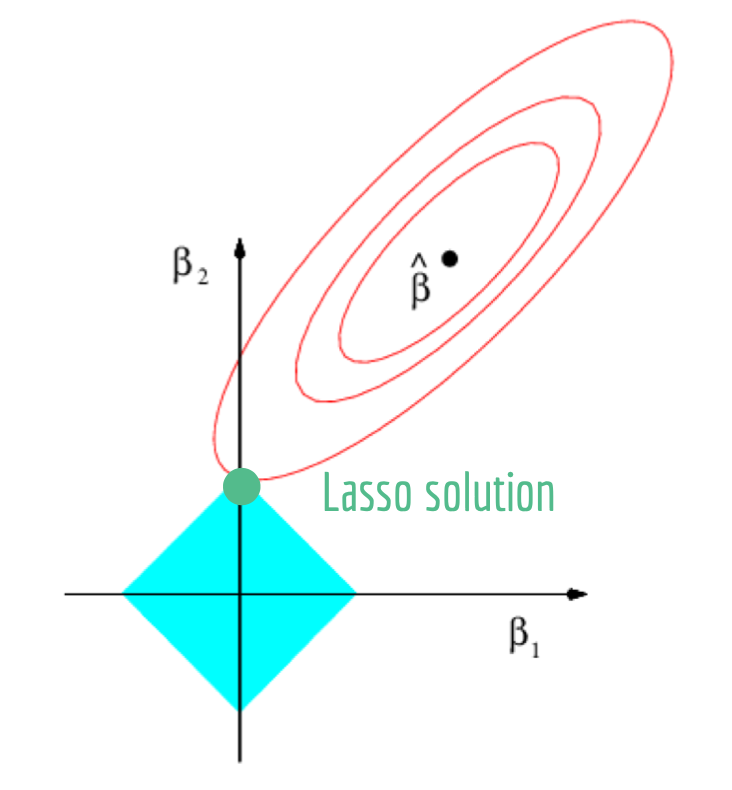
\includegraphics{lasso_vis.png}

\textbf{relationship between s and lambda???}

\hypertarget{selecting-the-tuning-parameter}{%
\subsubsection{Selecting the Tuning
Parameter}\label{selecting-the-tuning-parameter}}

\hypertarget{comparison-to-ridge-regression}{%
\subsubsection{Comparison to Ridge
Regression}\label{comparison-to-ridge-regression}}

Ridge regression is another technique that modifies the OLS framework by
constraining the values of the coefficients. Ridge regression is defined
as:
\[\text{argmin}_{\beta_j}\sum_{i=1}^n ( y_i +\beta_0 - \sum_{j=1}^p \beta_jx_{ij} )^2 + \color{red}{\lambda \sum_{j=1}^p (\beta_j)^2}\].
We can see that ridge regression is nearly identical to lasso; the only
difference is in the penalty term (shown above in red). Instead of
taking the absolute value of the coefficients, ridge regression squares
the coefficients. We can consider the constrained optimization
formulation of ridge regression, as we did for lasso: \[
\text{argmin}_{\beta_j}\sum_{i=1}^n ( y_i +\beta_0 - \sum_{j=1}^p \beta_jx_{ij} )^2  \text{; subject to }  \sum_{j=1}^p (\beta_j)^2 \le s.
\] With two predictors, the constraint region becomes a circle:
\(\beta_1^2 + \beta_2^2 \le s^2\). We can construct a very similar graph
to the one above:

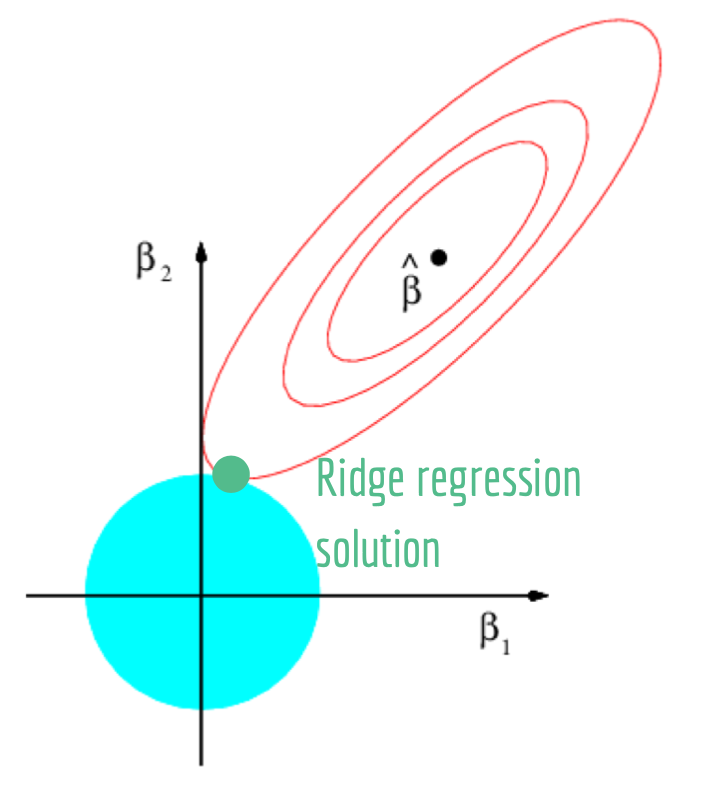
\includegraphics{ridge_vis.png} The only difference between lasso and
ridge regression are their constraint regions.

\hypertarget{variable-selection}{%
\subsubsection{Variable Selection}\label{variable-selection}}

\hypertarget{benefits-of-lasso-and-ridge-regression}{%
\subsubsection{Benefits of Lasso and Ridge
Regression}\label{benefits-of-lasso-and-ridge-regression}}

Both lasso and ridge regression are able to make more accurate
predictions than OLS in many contexts. Lasso and ridge regression are
often more accurate than OLS because they sacrifice a small increase in
bias for a significant reduction in variance. Both ridge regression and
lasso perform well in a variety of contexts, but the variable selection
property of lasso is a significant advantage. Lasso models have fewer
predictors, making them easier to interpret. Ridge regression, because
it includes every variable in the model, outperforms lasso when all of
the predictors are related to the outcome. On the other hand, lasso
outperforms ridge regression when only a few of the predictors are
related to the outcome. In the main results section, we will derived the
variance of OLS and ridge regression estimators and perform a simulation
to examine bias and variance in lasso estimators.

\hypertarget{main-results}{%
\subsection{Main Results}\label{main-results}}

\hypertarget{deriving-ols-ridge-regression-and-lasso-estimators}{%
\subsubsection{Deriving OLS, Ridge Regression and Lasso
Estimators}\label{deriving-ols-ridge-regression-and-lasso-estimators}}

\hypertarget{ols}{%
\paragraph{OLS}\label{ols}}

As described above, the OLS problem can be written as
\(\text{argmin}_{\boldsymbol\beta} (\mathbf{y} - \mathbf{X}\boldsymbol\beta)^\top(\mathbf{y} - \mathbf{X}\boldsymbol\beta)\).

We can derive the OLS estimate for \(\boldsymbol\beta\): \$\$

\begin{aligned}

&\text{argmin}_{\boldsymbol\beta} (\mathbf{y} - \mathbf{X}\boldsymbol\beta)^\top(\mathbf{y} - \mathbf{X}\boldsymbol\beta) \\

&= \frac{\partial}{\partial \boldsymbol\beta} (\mathbf{y}^\top \mathbf{y} - \mathbf{y}^\top\mathbf{X}\boldsymbol\beta  - \boldsymbol\beta^T\mathbf{X}^Ty + \boldsymbol\beta^\top \mathbf{X}^\top \mathbf{X} \boldsymbol\beta) \\ 


&= \frac{\partial}{\partial \boldsymbol\beta} (\mathbf{y}^\top \mathbf{y} - 2\mathbf{y}^\top\mathbf{X}\boldsymbol\beta + \boldsymbol\beta^\top \mathbf{X}^\top \mathbf{X} \boldsymbol\beta) \\

&= -2\mathbf{X}^\top\mathbf{y} + 2 \mathbf{X}^\top \mathbf{X} \boldsymbol\beta \\

0 &\stackrel{set}{=} -2\mathbf{X}^\top\mathbf{y} + 2 \mathbf{X}^\top \mathbf{X} \boldsymbol\beta \\

2 \mathbf{X}^\top \mathbf{X} \boldsymbol\beta &= 2\mathbf{X}^\top\mathbf{y} \\ 

(\mathbf{X}^T\mathbf{X})^{-1}\mathbf{X}^\top \mathbf{X} \boldsymbol\beta &= (\mathbf{X}^T\mathbf{X})^{-1} \mathbf{X}^\top\mathbf{y} \\ 

 \hat{\boldsymbol\beta}& = (\mathbf{X}^T\mathbf{X})^{-1} \mathbf{X}^\top\mathbf{y}

\end{aligned}

\$\$ \#\#\#\# Ridge Regression

In ridge regression, the formula we are trying to minimize is
\(\sum_{i=1}^n(y_i - \beta_0 - \sum_{j=1}^p\beta_j x_{ij})^2 + \lambda\sum_{j=1}^p \beta_j^2\).
We can write this in matrix notation as:
\((\mathbf{y} - \mathbf{X}\boldsymbol\beta)^\top(\mathbf{y} - \mathbf{X}\boldsymbol\beta) + \lambda \boldsymbol\beta^T\boldsymbol\beta\).
We can minimize this in much the same way as in OLS:

\$\$

\begin{aligned}

&\text{argmin}_{\boldsymbol\beta} (\mathbf{y} - \mathbf{X}\boldsymbol\beta)^\top(\mathbf{y} - \mathbf{X}\boldsymbol\beta) + \lambda \boldsymbol\beta^T\boldsymbol\beta \\ 

&= \frac{\partial}{\partial \boldsymbol\beta} (\mathbf{y}^\top \mathbf{y} - 2\mathbf{y}^\top\mathbf{X}\boldsymbol\beta + \boldsymbol\beta^\top \mathbf{X}^\top \mathbf{X} \boldsymbol\beta + \lambda \boldsymbol\beta^T\boldsymbol\beta) \\

&= -2\mathbf{X}^\top\mathbf{y} + 2 \mathbf{X}^\top \mathbf{X} \boldsymbol\beta + 2\lambda\boldsymbol\beta \\

0 &\stackrel{set}{=} -2\mathbf{X}^\top\mathbf{y} + 2 \mathbf{X}^\top \mathbf{X} \boldsymbol\beta + 2\lambda\boldsymbol\beta\\

\mathbf{X}^\top \mathbf{X} \boldsymbol\beta + \lambda\boldsymbol\beta &= \mathbf{X}^\top\mathbf{y} \\ 

(\mathbf{X}^\top \mathbf{X} + \lambda\mathbf{I}) \boldsymbol\beta &= \mathbf{X}^\top\mathbf{y} \\ 

(\mathbf{X}^\top \mathbf{X} + \lambda\mathbf{I}) (\mathbf{X}^\top \mathbf{X} + \lambda\mathbf{I}) ^{-1}\boldsymbol\beta &= \mathbf{X}^\top\mathbf{y}(\mathbf{X}^\top \mathbf{X} + \lambda\mathbf{I}) ^{-1}\\ 

\boldsymbol\beta &= \mathbf{X}^\top\mathbf{y}(\mathbf{X}^\top \mathbf{X} + \lambda\mathbf{I}) ^{-1}\\ 

\end{aligned}

\$\$

\hypertarget{considering-a-simple-case}{%
\paragraph{Considering a Simple Case}\label{considering-a-simple-case}}

We can consider a simple case: \(\mathbf{X}\) is a diagonal matrix with
1's on the diagonals and 0's on all the off diagonals, the number of
predictors equals the number of cases, and we force the intercept to go
through the origin. This case allows us simplify our OLS and ridge
regression estimators. For OLS, the solution is
\(\boldsymbol\beta = \mathbf{y}\) and for ridge regression the solution
becomes \(\boldsymbol\beta = \frac{\mathbf{y}}{1+\lambda}\). Applying
this simple case to find the estimators is helpful particularly for
Lasso. Unlike OLS and Ridge Regression, there is no closed form solution
for \(\boldsymbol\beta\) for Lasso. To derive any estimators for Lasso,
we must consider this simple case.

\hypertarget{lasso-estimators-in-a-simple-case}{%
\paragraph{Lasso Estimators in a Simple
Case}\label{lasso-estimators-in-a-simple-case}}

For lasso, we can not find a general closed form solution for
\(\boldsymbol\beta\), so we will derive the lasso estimates for
\(\boldsymbol\beta\) for the simple case described above. We will not
use matrix notation in order to easily apply the assumptions of our
simple case.

Remember that we can write the general form of lasso as:

\$\$

\begin{aligned}

\text{argmin}_{\beta}\sum_{i=1}^n(y_i - \beta_0 - \sum_{j=1}^p\beta_j x_{ij})^2 + \lambda\sum_{j=1}^p |\beta_j|

\end{aligned}

\$\$ If we apply our simplifying assumptions, we can write:

\$\$

\begin{aligned}

\text{argmin}_{\beta}\sum_{j=1}^p(y_i - \beta_1)^2 + \lambda|\beta_1| 

\end{aligned}

\$\$

With these assumptions, we can find a closed form solution for
\(\beta\):

\$\$

\begin{aligned}

&\text{argmin}_{\beta}(y_i - \beta_1)^2 + \lambda|\beta_1| \\ 

&= \frac{\partial}{\partial \beta} \left( (y_j - \beta_1)^2 + \lambda|\beta_1| \right) \\

&= \frac{\partial}{\partial \beta} \left( y_j^2 - 2y_j\beta_1 + \beta_1^2 + \lambda|\beta_1| \right) \\

&=  - 2y_j + 2\beta_1 + \lambda sign(\beta_1) \\

\end{aligned}

\$\$ To solve for \(\beta_1\), we must consider different regions: (1)
when \(\beta_1 < 0\), (2) when \(\beta_1 > 0\) and (3) when
\(\beta_1 = 0\).

\begin{enumerate}
\def\labelenumi{(\arabic{enumi})}
\tightlist
\item
  when \(\beta_1 < 0\) or when \(y_j < - \lambda/2\):
\end{enumerate}

\$\$

\begin{aligned}

0 &\stackrel{set}{=} - 2y_j + 2\beta_1 - \lambda \\

\beta_1 &= y_j + \lambda/2 \\

\end{aligned}

\[
(2) when $\beta_1 > 0$ or when $y_j > \lambda/2$: 
\]

\begin{aligned}

0 &\stackrel{set}{=} - 2y_j + 2\beta_1 + \lambda \\

\beta_1 &= y_j - \lambda/2 \\

\end{aligned}

\[
(3) when $\beta_1 = 0$ ASK KELSEY
\]

\text{when } \beta\_1 = 0 \text{ or when } \textbar y\_i\textbar{}
\le \lambda/2 : \textbackslash{}

0

\$\$

\hypertarget{visualizing-the-simple-case-estimators}{%
\paragraph{Visualizing the Simple Case
Estimators}\label{visualizing-the-simple-case-estimators}}

The graph below shows the simple case coefficient estimates for OLS,
ridge regression and lasso as a function of the data \(y_j\). We can see
from that graph, and from the equations derived above, that ridge
regression scales the coefficient estimates by the same factor,
\(1/(1+\lambda)\), regardless of the value of \(y_j\). Since it is
impossible to divide a non-zero number by any value and get 0, ridge
regression cannot set any coefficient to zero unless it is already 0.
However, lasso performs shrinkage in a different way, allowing some
coefficients to be 0. Lasso changes the values of the coefficients by
adding or subtracting \(\lambda/2\), depending on the corresponding
\(y_j\). If \(y_j\) is inside the region \((-\lambda/2, \lambda/2)\),
the coefficient is shrunk to 0.

\begin{Shaded}
\begin{Highlighting}[]
\FunctionTok{library}\NormalTok{(ggplot2)}
\NormalTok{lambda }\OtherTok{\textless{}{-}} \DecValTok{5}
\NormalTok{ols }\OtherTok{\textless{}{-}} \ControlFlowTok{function}\NormalTok{(x) x}
\NormalTok{ridge }\OtherTok{\textless{}{-}} \ControlFlowTok{function}\NormalTok{(x) x}\SpecialCharTok{/}\NormalTok{(}\DecValTok{1}\SpecialCharTok{+}\NormalTok{lambda)}
\NormalTok{lasso }\OtherTok{\textless{}{-}}\ControlFlowTok{function}\NormalTok{(x) }\FunctionTok{ifelse}\NormalTok{(x }\SpecialCharTok{\textgreater{}}\NormalTok{ lambda}\SpecialCharTok{/}\DecValTok{2}\NormalTok{, x}\SpecialCharTok{{-}}\NormalTok{lambda}\SpecialCharTok{/}\DecValTok{2}\NormalTok{,}
   \FunctionTok{ifelse}\NormalTok{(x }\SpecialCharTok{\textless{}} \SpecialCharTok{{-}}\NormalTok{lambda}\SpecialCharTok{/}\DecValTok{2}\NormalTok{, x}\SpecialCharTok{+}\NormalTok{lambda}\SpecialCharTok{/}\DecValTok{2}\NormalTok{, }
   \FunctionTok{ifelse}\NormalTok{( }\SpecialCharTok{{-}}\NormalTok{lambda}\SpecialCharTok{/}\DecValTok{2} \SpecialCharTok{\textless{}=}\NormalTok{ x }\SpecialCharTok{\&}\NormalTok{ x }\SpecialCharTok{\textless{}=}\NormalTok{ lambda}\SpecialCharTok{/}\DecValTok{2}\NormalTok{, }\DecValTok{0}\NormalTok{, }\DecValTok{0}\NormalTok{)))}


\FunctionTok{ggplot}\NormalTok{() }\SpecialCharTok{+}
  \FunctionTok{xlim}\NormalTok{(}\SpecialCharTok{{-}}\DecValTok{10}\NormalTok{, }\DecValTok{10}\NormalTok{)}\SpecialCharTok{+}
  \FunctionTok{geom\_function}\NormalTok{(}\AttributeTok{fun =}\NormalTok{ ols,}
                \FunctionTok{aes}\NormalTok{(}\AttributeTok{color =} \StringTok{\textquotesingle{}OLS\textquotesingle{}}\NormalTok{),}
                \AttributeTok{linetype =} \StringTok{"dashed"}\NormalTok{) }\SpecialCharTok{+}
  \FunctionTok{geom\_function}\NormalTok{ (}\AttributeTok{fun =}\NormalTok{ ridge,}
                 \FunctionTok{aes}\NormalTok{(}\AttributeTok{color =} \StringTok{\textquotesingle{}Ridge\textquotesingle{}}\NormalTok{),}
                 \AttributeTok{lwd =} \FloatTok{1.2}\NormalTok{)}\SpecialCharTok{+}
  \FunctionTok{geom\_function}\NormalTok{(}\AttributeTok{fun =}\NormalTok{ lasso,}
                \FunctionTok{aes}\NormalTok{(}\AttributeTok{color =} \StringTok{\textquotesingle{}Lasso\textquotesingle{}}\NormalTok{),}
                \AttributeTok{lwd =} \FloatTok{1.2}\NormalTok{) }\SpecialCharTok{+}
  \FunctionTok{theme\_bw}\NormalTok{()}\SpecialCharTok{+}
  \FunctionTok{theme}\NormalTok{(}\AttributeTok{panel.grid.minor.x =} \FunctionTok{element\_blank}\NormalTok{(),}
        \AttributeTok{panel.grid.minor.y =} \FunctionTok{element\_blank}\NormalTok{())}\SpecialCharTok{+}
  \FunctionTok{scale\_color\_manual}\NormalTok{(}\AttributeTok{name =} \StringTok{\textquotesingle{}Models\textquotesingle{}}\NormalTok{,}
                     \AttributeTok{breaks =} \FunctionTok{c}\NormalTok{(}\StringTok{\textquotesingle{}OLS\textquotesingle{}}\NormalTok{, }\StringTok{\textquotesingle{}Ridge\textquotesingle{}}\NormalTok{, }\StringTok{\textquotesingle{}Lasso\textquotesingle{}}\NormalTok{),}
                     \AttributeTok{values =} \FunctionTok{c}\NormalTok{(}\StringTok{\textquotesingle{}OLS\textquotesingle{}}\OtherTok{=}\StringTok{\textquotesingle{}gray54\textquotesingle{}}\NormalTok{, }\StringTok{\textquotesingle{}Ridge\textquotesingle{}}\OtherTok{=}\StringTok{\textquotesingle{}olivedrab3\textquotesingle{}}\NormalTok{, }\StringTok{\textquotesingle{}Lasso\textquotesingle{}}\OtherTok{=}\StringTok{\textquotesingle{}tan2\textquotesingle{}}\NormalTok{))}\SpecialCharTok{+}
  \FunctionTok{labs}\NormalTok{(}\AttributeTok{y =} \StringTok{"Coefficient Estimates"}\NormalTok{, }\AttributeTok{x =} \StringTok{"yj"}\NormalTok{)}
\end{Highlighting}
\end{Shaded}

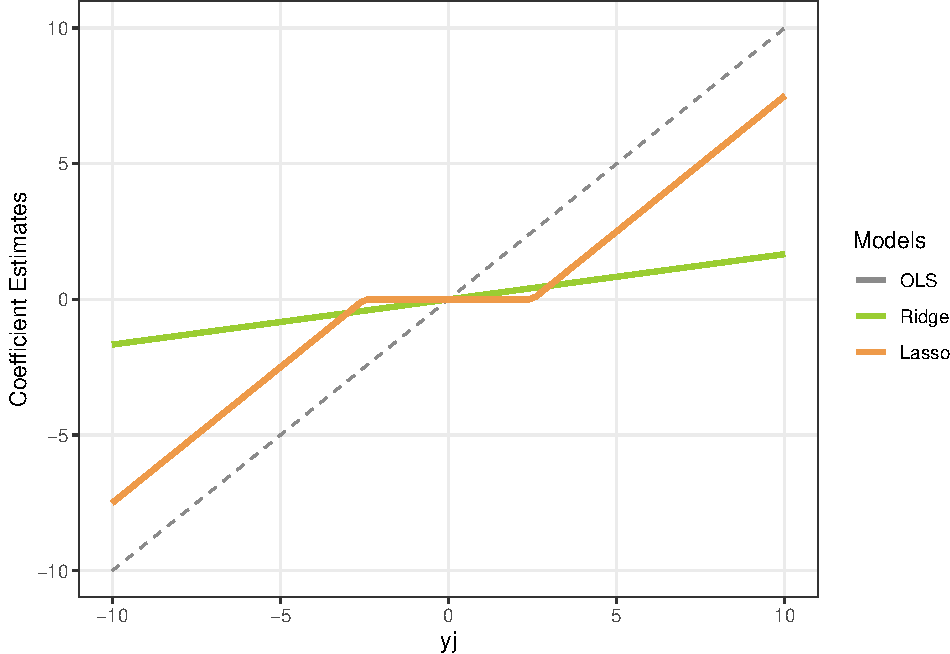
\includegraphics{Final-Project_files/figure-latex/unnamed-chunk-1-1.pdf}

\hypertarget{deriving-bias-and-variance-of-ols-and-ridge-regression-estimators}{%
\subsection{Deriving Bias and Variance of OLS and Ridge Regression
Estimators}\label{deriving-bias-and-variance-of-ols-and-ridge-regression-estimators}}

\hypertarget{ols-1}{%
\subsubsection{OLS}\label{ols-1}}

\hypertarget{bias}{%
\paragraph{Bias}\label{bias}}

We will assume that
\(\mathbf{y} = \mathbf{X}\boldsymbol\beta + \boldsymbol\epsilon\) and
that \(E[\boldsymbol\epsilon] = \mathbf{0}\). We can show that the least
squares estimator
\(\hat{\boldsymbol\beta} = (\mathbf{X}^T\mathbf{X})^{-1} \mathbf{X}^\top\mathbf{y}\)
is an unbiased estimator of \(\boldsymbol\beta\):

\$\$

\begin{aligned}

E[\hat{\boldsymbol\beta}_{OLS}] &= E[(\mathbf{X}^T\mathbf{X})^{-1} \mathbf{X}^\top\mathbf{y}]\\
&= (\mathbf{X}^T\mathbf{X})^{-1} \mathbf{X}^\top E[\mathbf{y}], \text{ since X is fixed} \\
&= (\mathbf{X}^T\mathbf{X})^{-1} \mathbf{X}^\top E[\mathbf{X}\boldsymbol\beta  + \boldsymbol\epsilon], \text{ by assumption}\\
&= (\mathbf{X}^T\mathbf{X})^{-1} \mathbf{X}^\top (\mathbf{X}\boldsymbol\beta  + E[\boldsymbol\epsilon])\\
&= (\mathbf{X}^T\mathbf{X})^{-1} \mathbf{X}^\top (\mathbf{X}\boldsymbol\beta  + 0), \text{ by assumption}\\
&=(\mathbf{X}^T\mathbf{X})^{-1} (\mathbf{X}^\top\mathbf{X})\boldsymbol\beta \\
&= \boldsymbol\beta
\end{aligned}

\$\$ \#\#\#\# Variance We will assume that
\(\mathbf{y} = \mathbf{X}\boldsymbol\beta + \boldsymbol\epsilon\),
\(E[\boldsymbol\epsilon] = \mathbf{0}\) and that
\(Var[\boldsymbol\epsilon] = \sigma^2 \mathbf{I}\). We can show that the
variance of the least squares estimator
\(\hat{\boldsymbol\beta} = (\mathbf{X}^T\mathbf{X})^{-1} \mathbf{X}^\top\mathbf{y}\)
is
\(Var[\hat{\boldsymbol\beta}] = \sigma^2(\mathbf{X}^T\mathbf{X})^{-1}\):

\$\$

\begin{aligned}

Var[\hat{\boldsymbol\beta}_{OLS}] &= Var[(\mathbf{X}^T\mathbf{X})^{-1} \mathbf{X}^\top\mathbf{y}]\\

&= (\mathbf{X}^T\mathbf{X})^{-1} \mathbf{X}^\top Var[\mathbf{y}]((\mathbf{X}^T\mathbf{X})^{-1} \mathbf{X}^\top)^\top, \text{ since } Var(\mathbf{Ax}) = \mathbf{A}Var(\mathbf{x})\mathbf{A}^\top \\

&= (\mathbf{X}^T\mathbf{X})^{-1} \mathbf{X}^\top Var[\mathbf{y}] \mathbf{X}(\mathbf{X}^T\mathbf{X})^{-1}, \text{ since } (\mathbf{AB})^\top = \mathbf{B}^\top\mathbf{A}^\top \text{ and } (\mathbf{A}^{-1})^\top = (\mathbf{A}^\top)^{-1} \\

&= (\mathbf{X}^T\mathbf{X})^{-1} \mathbf{X}^\top Var[\mathbf{X}\boldsymbol\beta  + \boldsymbol\epsilon] \mathbf{X}(\mathbf{X}^T\mathbf{X})^{-1}, \text{ by assumption}\\

&= (\mathbf{X}^T\mathbf{X})^{-1} \mathbf{X}^\top Var[\boldsymbol\epsilon] \mathbf{X}(\mathbf{X}^T\mathbf{X})^{-1}, \text{ since } \mathbf{X} \text{ and } \boldsymbol{\beta} \text{ are fixed}\\

&= (\mathbf{X}^T\mathbf{X})^{-1} \mathbf{X}^\top (\sigma^2\mathbf{I}) \mathbf{X}(\mathbf{X}^T\mathbf{X})^{-1}, \text{ by assumption} \\

&= \sigma^2(\mathbf{X}^T\mathbf{X})^{-1} (\mathbf{X}^\top \mathbf{X})(\mathbf{X}^T\mathbf{X})^{-1} \\

&= \sigma^2(\mathbf{X}^T\mathbf{X})^{-1} \\

\end{aligned}

\$\$

\hypertarget{ridge-regression}{%
\subsubsection{Ridge Regression}\label{ridge-regression}}

\hypertarget{bias-1}{%
\paragraph{Bias}\label{bias-1}}

We will assume that
\(\mathbf{y} = \mathbf{X}\boldsymbol\beta + \boldsymbol\epsilon\) and
that \(E[\boldsymbol\epsilon] = \mathbf{0}\). We can show that the ridge
regression estimator
\(\boldsymbol\beta = (\mathbf{X}^\top \mathbf{X} + \lambda\mathbf{I}) ^{-1}\mathbf{X}^\top\mathbf{y}\)
is a biased estimator of \(\boldsymbol\beta\):

\$\$

\begin{aligned}

E[\hat{\boldsymbol\beta}_{ridge}] &= E[(\mathbf{X}^\top \mathbf{X} + \lambda\mathbf{I}) ^{-1}\mathbf{X}^\top\mathbf{y}]\\

&= E[(\mathbf{X}^\top \mathbf{X} + \lambda\mathbf{I}) ^{-1}\mathbf{X}^\top (\mathbf{X}\boldsymbol\beta + \boldsymbol\epsilon)], \text{ by assumption} \\

&= E[(\mathbf{X}^\top \mathbf{X} + \lambda\mathbf{I}) ^{-1}\mathbf{X}^\top (\mathbf{X}\boldsymbol\beta) + (\mathbf{X}^\top \mathbf{X} + \lambda\mathbf{I}) ^{-1}\mathbf{X}^\top (\boldsymbol\epsilon)] \\

&= E[(\mathbf{X}^\top \mathbf{X} + \lambda\mathbf{I}) ^{-1}\mathbf{X}^\top (\mathbf{X}\boldsymbol\beta)] + E[(\mathbf{X}^\top \mathbf{X} + \lambda\mathbf{I}) ^{-1}\mathbf{X}^\top (\boldsymbol\epsilon)] \\

&= (\mathbf{X}^\top \mathbf{X} + \lambda\mathbf{I}) ^{-1}\mathbf{X}^\top (\mathbf{X}\boldsymbol\beta) + (\mathbf{X}^\top \mathbf{X} + \lambda\mathbf{I}) ^{-1}\mathbf{X}^\top E[(\boldsymbol\epsilon)], \text{ since } \mathbf{X} \text{ and } \boldsymbol{\beta} \text{ are fixed} \\

&= (\mathbf{X}^\top \mathbf{X} + \lambda\mathbf{I}) ^{-1}\mathbf{X}^\top (\mathbf{X}\boldsymbol\beta) + (\mathbf{X}^\top \mathbf{X} + \lambda\mathbf{I}) ^{-1}\mathbf{X}^\top (0), \text{ by assumption } \\

&= (\mathbf{X}^\top \mathbf{X} + \lambda\mathbf{I}) ^{-1}\mathbf{X}^\top \mathbf{X}\boldsymbol\beta  \\

\end{aligned}

\$\$ Since
\(E[\hat{\boldsymbol\beta}_{ridge}] = (\mathbf{X}^\top \mathbf{X} + \lambda\mathbf{I}) ^{-1}\mathbf{X}^\top \mathbf{X}\boldsymbol\beta\),
the ridge regression estimator for \(\boldsymbol{\beta}\) will always be
biased, unless \(\lambda = 0\). If \(\lambda = 0\), the ridge regression
estimator is equal to the OLS estimator, which we showed above is
unbiased.

\hypertarget{variance}{%
\subsubsection{Variance}\label{variance}}

We will assume that
\(\mathbf{y} = \mathbf{X}\boldsymbol\beta + \boldsymbol\epsilon\),
\(E[\boldsymbol\epsilon] = \mathbf{0}\) and that
\(Var[\boldsymbol\epsilon] = \sigma^2 \mathbf{I}\). We can show that the
variance of the ridge regression estimator is
\(\sigma^2(\mathbf{X}^\top \mathbf{X} + \lambda\mathbf{I}) ^{-1}\mathbf{X}^\top \mathbf{X} (\mathbf{X}^\top \mathbf{X} + \lambda\mathbf{I})^{-1}\):

\$\$

\begin{aligned}
Var[\hat{\boldsymbol\beta}_{ridge}] &= Var((\mathbf{X}^\top \mathbf{X} + \lambda\mathbf{I}) ^{-1}\mathbf{X}^\top\mathbf{y})\\

&= (\mathbf{X}^\top \mathbf{X} + \lambda\mathbf{I}) ^{-1}\mathbf{X}^\top Var(\mathbf{y}) ((\mathbf{X}^\top \mathbf{X} + \lambda\mathbf{I}) ^{-1}\mathbf{X}^\top)^\top, \text{ since } Var(\mathbf{Ax}) = \mathbf{A}Var(\mathbf{x})\mathbf{A}^\top \\

&= (\mathbf{X}^\top \mathbf{X} + \lambda\mathbf{I}) ^{-1}\mathbf{X}^\top Var(\mathbf{X}\boldsymbol\beta + \boldsymbol\epsilon) ((\mathbf{X}^\top \mathbf{X} + \lambda\mathbf{I}) ^{-1}\mathbf{X}^\top)^\top, \text{ by assumption } \\

&= (\mathbf{X}^\top \mathbf{X} + \lambda\mathbf{I}) ^{-1}\mathbf{X}^\top (Var(\mathbf{X}\boldsymbol\beta) + Var(\boldsymbol\epsilon)) ((\mathbf{X}^\top \mathbf{X} + \lambda\mathbf{I}) ^{-1}\mathbf{X}^\top)^\top \\

&= (\mathbf{X}^\top \mathbf{X} + \lambda\mathbf{I}) ^{-1}\mathbf{X}^\top Var(\boldsymbol\epsilon) ((\mathbf{X}^\top \mathbf{X} + \lambda\mathbf{I}) ^{-1}\mathbf{X}^\top)^\top, \text{ since } \mathbf{X} \text{ and } \boldsymbol{\beta} \text{ are fixed} \\

&= (\mathbf{X}^\top \mathbf{X} + \lambda\mathbf{I}) ^{-1}\mathbf{X}^\top (\sigma^2\mathbf{I}) ((\mathbf{X}^\top \mathbf{X} + \lambda\mathbf{I}) ^{-1}\mathbf{X}^\top)^\top, \text{ by assumption }  \\

&= \sigma^2(\mathbf{X}^\top \mathbf{X} + \lambda\mathbf{I}) ^{-1}\mathbf{X}^\top) ((\mathbf{X}^\top \mathbf{X} + \lambda\mathbf{I}) ^{-1}\mathbf{X}^\top)^\top \\

&= \sigma^2(\mathbf{X}^\top \mathbf{X} + \lambda\mathbf{I}) ^{-1}\mathbf{X}^\top \mathbf{X} ((\mathbf{X}^\top \mathbf{X} + \lambda\mathbf{I}) ^{-1})^\top \\

& = \sigma^2(\mathbf{X}^\top \mathbf{X} + \lambda\mathbf{I}) ^{-1}\mathbf{X}^\top \mathbf{X} (\mathbf{X}^\top \mathbf{X} + \lambda\mathbf{I})^{-1} \\

\end{aligned}

\$\$ We can show that the variance of the ridge regression estimator is
equal to the variance of the OLS estimator when \(\lambda = 0\):

\$\$

\begin{aligned}

Var[\hat{\boldsymbol\beta}_{ridge}] \text{ when } \lambda = 0: \\
&= \sigma^2(\mathbf{X}^\top \mathbf{X} + 0\mathbf{I}) ^{-1}\mathbf{X}^\top \mathbf{X} (\mathbf{X}^\top \mathbf{X} + 0\mathbf{I})^{-1} \\
&= \sigma^2(\mathbf{X}^\top \mathbf{X}) ^{-1}\mathbf{X}^\top \mathbf{X} (\mathbf{X}^\top \mathbf{X})^{-1} \\
&= \sigma^2(\mathbf{X}^\top \mathbf{X}) ^{-1} = Var[\hat{\boldsymbol\beta}_{OLS}]

\end{aligned}

\$\$ Importantly, the variance of the ridge regression estimator is
always smaller than the variance of the OLS estimator when
\(\lambda>0\). To see that this is true, we can consider the case when
\(\mathbf{X}\) is a 1 by 1 matrix with value 1 ({[}1{]}) and
\(\lambda = 1\):

\$\$

\begin{aligned}

Var[\hat{\boldsymbol\beta}_{ridge}] &= \sigma^2(\mathbf{X}^\top \mathbf{X} + \lambda\mathbf{I}) ^{-1}\mathbf{X}^\top \mathbf{X} (\mathbf{X}^\top \mathbf{X} + \lambda\mathbf{I})^{-1} \\

&= \sigma^2(1 *1 + 1) ^{-1}1*1 (1*1 + 1)^{-1} \\

&= \sigma^2(2) ^{-1}(2)^{-1} \\

&= \frac{\sigma^2}{4} 

\end{aligned}

\[
\]

\begin{aligned}

Var[\hat{\boldsymbol\beta}_{OLS}] &= \sigma^2(\mathbf{X}^T\mathbf{X})^{-1} \\

&= \sigma^2(1 *1) ^{-1} \\

&= \frac{\sigma^2}{1} = \sigma^2

\end{aligned}

\$\$ From this simple case, we can see that
\(Var[\hat{\boldsymbol\beta}_{ridge}]\) is smaller than
\(Var[\hat{\boldsymbol\beta}_{OLS}]\). This holds true for all cases
when \(\lambda>0\), but the proof of that is beyond the scope of this
project.

\hypertarget{lasso-1}{%
\subsubsection{Lasso}\label{lasso-1}}

Lasso, unlike OLS and ridge regression, does not have closed form
solutions for the bias and variance of its estimator. To examine the
bias and variance of lasso estimators, we constructed a simulation and
we discuss the results of the simulation in the next section.

\hypertarget{simulation}{%
\subsection{Simulation}\label{simulation}}

\hypertarget{references}{%
\subsection{References}\label{references}}

\begin{enumerate}
\def\labelenumi{\arabic{enumi}.}
\item
  Gunes, Funda. ``Penalized Regression Methods for Linear Models in
  SAS/STAT®.'' SAS Institute, Inc.~2015, p.~1.
\item
  James, Gareth, et al.~``The Lasso.'' An Introduction to Statistical
  Learning: with Applications in R. New York, Springer, 2013.
\item
  ``Lasso (statistics).'' Wikipedia. Wikimedia Foundation, 13 Feb.~2022,
  \url{https://en.wikipedia.org/wiki/Lasso_(statistics)}
\item
  Ranstam, J. Cook, J. A. ``LASSO regression.'' British Journal of
  Surgery, vol.~105, iss. 10, 2018, p.~1348.
\item
  Tibshirani, Robert. ``Regression Shrinkage and Selection via the
  Lasso.'' Journal of the Royal Statistical Society. Series B
  (Methodological), vol.~58, no. 1, 1996, pp.~267--88.
\end{enumerate}

\end{document}
